%------------------------------------------------------------------------------
\chapter{Conclusions and Future work}
\label{ch:conclusions}

\section{Conclusions}

Without a reference it is quite difficult to judge what looks like real fire and what does not.

Volume tracing is quite computationally expensive, intrinsic problems due to gamma correction and limited rgb space on the monitor.
Fire actually saturates our cones and the visual adaptation is just an aproximation of that.

The quality of the final image depends significantly on the shape of the fire, ..., Pegoraro images look worse than Hong, even though Hong is using a simpler rendering technique.

 

\section{Future Work}

An interesting area of future work involves automatically setting the shader parameters for a given scene.
There are at least two paths that be used to give a good parameter estimation, if we have captured data.
The methods are, gradient descent using image derivatives or reconstructing the spectrum which produced the cameras RGB responses.
Both techniques will be explained in greater detail in the Sections~\ref{sec:image_differences} and~\ref{sec:spectrum_reconstruction}.

A common line of work in the computer graphics community is the development of importance sampling for a bxdf rendering models~\cite{Lawrence:2004},~\cite{Ou:2012} and~\cite{Wang:2014}.
The core idea is to sample more often the values that contribute more to the final image, by means of a biased distribution instead of an uniform sampling scheme.
In our implementation the emitted radiance $L_e$ is uniformly sampled, and in the general case the $\omegam_i$ directions for in-scattering light $L_i$ would have been naively sampled as well.
In order to design a ``good" biased distribution, prior knowledge of the location of the important regions is needed. 
For $L_e$ and $L_i$ we have some intuitive insight on were would such regions lie, samples whose origin is close to the interest point should have greater contributions, as the influence of further ones will be diminished by the light distance falloff effect.
Another factor which must be considered is the relative intensity emitted at source by a sample, as it is expected that brighter points will have larger contributions. 

\subsection{Image differences}
\label{sec:image_differences}

Given a ground truth captured image $I_f$, we would like to transform an image $I_0$, rendered with our method, so that it resembles $I_f$.
Formally the transformation is defined as

\begin{equation}
I_{i+1} = t(I_i,~d(I_i,~I_f)),
\end{equation}

where $I_i$ is the image in the $i^{th}$ step, $d$ is an image difference function, and $t$ is a function that transform $I_i$ in the direction of the gradient given by $d$.
There are several terms in the aforementioned equation that can be explored in more detail.
A number of image difference filters have been proposed, such as the Sobel and the Scharr filters.
The transformation function $t$ must convert from image derivatives space, to the physical parameter space that our shaders use, temperature, density, light falloff rate, etc.
The simplest technique to compute the next step in the parameter space would be gradient descent.
As there are several parameters to explore, and their behaviour is non-linear, it is reasonable to expect that the function will have a number of local minima. 
Thus, requiring more advanced optimization methods, such as genetic programming.

\subsection{Spectrum reconstruction}
\label{sec:spectrum_reconstruction}

In a captured image $I_f$, each pixel stores the RGB values that were measured by the sensor at that position.
When the camera is exposed to a spectral signal, the spectrum is collapsed to RGB space using the sensor spectral sensitivity curves for each color, the curves are shown in Figure~\ref{fig:camera_sensitivity}.
In continuous form, the collapsing of the signal is driven by

\begin{figure}[htbp!]
\centering
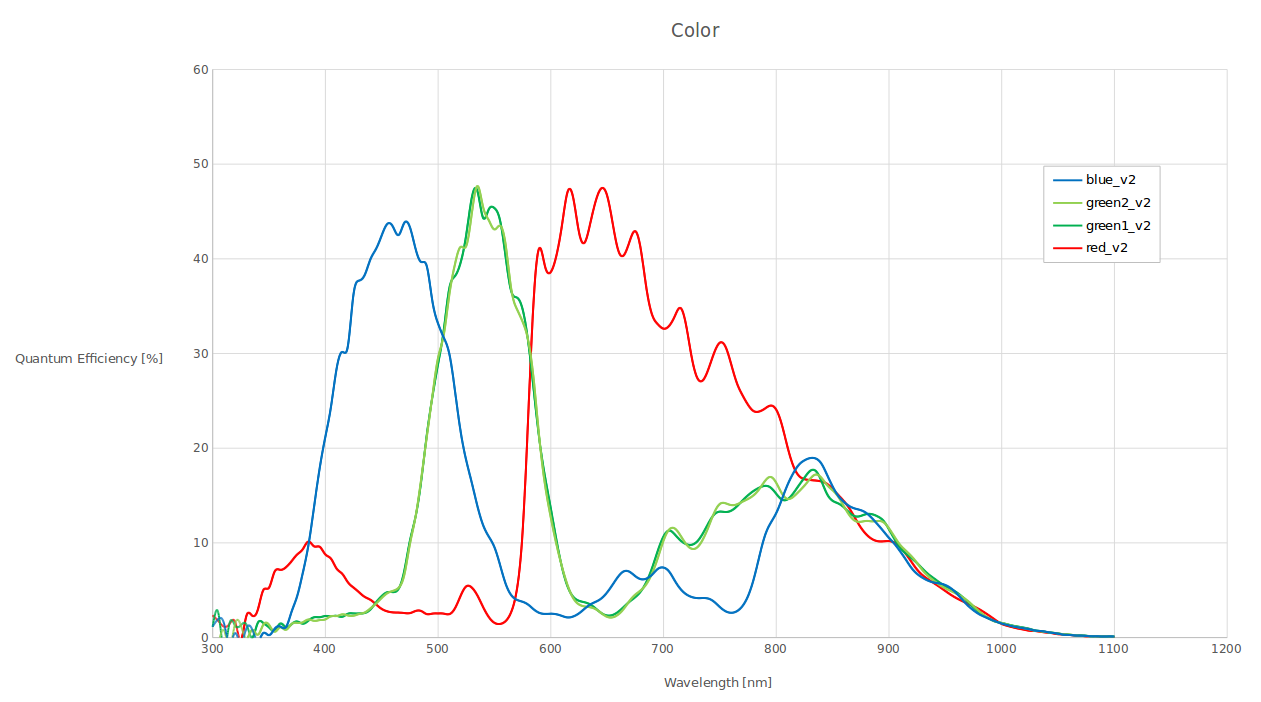
\includegraphics[width=0.8\textwidth]{img/camera_sensitivity}
	\caption{Spectral sensitivity curves for the sensors in our cameras.}
	\label{fig:camera_sensitivity}
\end{figure}

\begin{equation}
\begin{split}
r &= \int i(\lambda) s_r(\lambda) d \lambda, \\
g &= \int i(\lambda) s_g(\lambda) d \lambda, \\
b &= \int i(\lambda) s_b(\lambda) d \lambda,
\end{split}
\label{eq:spectrum_collapse_cont}
\end{equation}

where $r$, $g$ and $b$ are the output coefficients, $i(\lambda)$ is the input spectrum, $s_r(\lambda)$, $s_g(\lambda)$ and $s_b(\lambda)$ are the spectral sensitivity curves and $\lambda$ is a wavelength number.
Discretized for $n$ samples the previous equation can be written as  

\begin{equation}
\begin{bmatrix}
r \\
g \\
b
\end{bmatrix}
= 
\begin{bmatrix}
s_r(\lambda_0) & s_r(\lambda_1) & \cdots & s_r(\lambda_n) \\
s_g(\lambda_0) & s_g(\lambda_1) & \cdots & s_g(\lambda_n) \\
s_b(\lambda_0) & s_b(\lambda_1) & \cdots & s_b(\lambda_n) 
\end{bmatrix}
\begin{bmatrix}
i(\lambda_0) \\
i(\lambda_1) \\
\vdots \\
i(\lambda_n) 
\end{bmatrix}.
\label{eq:spectrum_collapse_disc}
\end{equation}

If the original signal $i(\lambda)$ were to be reconstructed, the physical parameters could be computed using the equations presented in Chapter~\ref{ch:methodology}.
An image rendered with those parameters would closely resemble the original data.
The main challenge in this situation lies in the highly underconstrained nature of the problem, $n$ unknowns in $i(\lambda)$ are to be solved with only three equations from $r$, $g$ and $b$.
Fortunately, several methods have been proposed,~\cite{Smits:1999},~\cite{Sun2001} and~\cite{Drew:2003}, to compute an approximation of $i(\lambda)$ using optimization techniques with a set of prior constrains, such as smooth spectral curves and spatial coherency within the image.

